\section{Styrhandske}
Styrhandsken innefattar en handske med flexsensorer, ledlampor??, en mikrokontroller, kalibreringsknappar och en bluetoothmodul.
\begin{figure}[H]
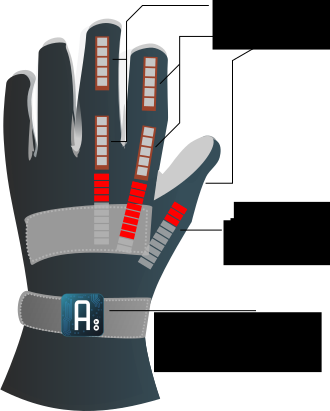
\includegraphics[height=0.5\textheight]{img/kontrollhandske}
\caption{Konceptskiss över styrhandsken}
\label{handske}
\end{figure}

Bilden måste bytas ut om vi inte får på led. För att intuitivt reglera robothanden används en arbetshandske som användaren bär på sin hand. Handsken är gjord av textil och på tummen, långfingret och pekfingret är det två flexsensorer enligt Figur \ref{handske}. Flexsensorerna är av modellen SEN-10264 och ändrar resistans beroende på hur böjda de är. Styrhandsken sköter det som händer i punkt 1-3 enligt Figur \ref{flodesschema} via handskens mikrokontroller som kommunicerar med robothandens mikrokontroller via bluetooth.

\subsection{Mikrokontroller }
\label{sec:mikro}
För kontrollhandsken används en 8 bitars Arduino Micro. Eftersom alla beräkningar kommer att ske i robothanden är mikrokontrollen i handskens enda uppgift att överföra signaler. Storleken och strömförbrukningen är här av större vikt.

En 32 bitars Arduino Due används för robothanden. Eftersom alla reglerberäkning sker i robothanden i sig, är prestanda viktigt. 32 bitar är viktigt för att effektivt kunna använda fixpunkttal\footnote{Tal som har en fast decimalposition. Decimalens plats måste skötas manuellt} med tillräcklig precision.



\subsection{Bluetooth}
För att möjliggöra kommunikation trådlöst mellan kontrollhandsken och robothanden används två prototyp-versioner av \emph{Bluetooth Mate Silver}. Enheten är godkänd för Bluetooth klass 2, vilket bl a innebär låg strömförbrukning (genomsnittligt 2.5mW vid aktiv användning) och överföringar på upp till 10m, vilket anses vara tillräckligt för att klara kravet på 5m i praktiska förhållanden.

Bluetooth-protokollet är ett paketförmedlande nätverk, vilket innebär att information skickas i diskreta paket. Varje paket innehåller metadata
\footnote{Data som beskriver information, som mottagaradress och felkorrigerande kod}
och \emph{payload}
\footnote{Datan i sig som ska överföras}.
Bluetooth-enheten har en överföringskapacitet på 115200bps, inkluderat metadata.


\begin{figure}[ht]
\includegraphics[width=0.3\textwidth]{img/bluetooth_mate_silver.jpg}
\caption{Bluetooth Mate Silver enhet.}
\end{figure}

\begin{figure}[htb]
\includegraphics[width=0.3\textwidth]{img/arduino_micro}
\caption{Ardunio Micro. Används för kontrollhandsken.}
\end{figure}

\subsection{Trådlös kommunikation}

\subsection{Signalbehandling}
Från flexsensorerna samplas en varierande analog spänning med en frekvens på 100 Hz. Signalen diskretireras sedan till upplösning av 10 bitar. I uppmätta mätvärdet finns det diverse störningar. Det är inte önskvärt att störningarna överförs till robothanden, eftersom servomotorerna i robothanden då konstant skulle ändra läge, vilket leder till en hackig upplevelse för användaren, slitage på servomotorerna, och extra strömförbrukning.

\begin{figure}[htb]
\includegraphics{img/filter/flex_raw.pdf}
\caption{De sex flexsensorerna uppmätta under 8.0s med en samplingsfrekvens på 100Hz när handen greppar ett objekt.}
\label{fig:rawflex}
\end{figure}

\begin{figure}[htb]
\includegraphics{img/filter/flex_fourier.pdf}
\caption{Diskret fouriertransform av signalerna från figur~\ref{fig:rawflex}.}
\end{figure}


\begin{figure}[htb]
\includegraphics{img/filter/flex_filtered.pdf}
\caption{Signalerna från figur~\ref{fig:rawflex} filtrerade med ett Butterworth-filter av första ordningen med en brytningsfrekvens på $f=\unit[15]{Hz}$.}
\end{figure}



För att filtera signalen används ett \emph{Butterworth-filter} av första ordningen. Butterworth filter filterar


\section{Algoritmer}
Här presenteras de styralgortimter som bestämmer hur handen beter sig när den följer användarens input samt identifierar och greppar objekt. 
\subsection{Objektidentifiering}
\begin{figure}[H]
EN BILD SOM FÖRKLARAR DETTA, SAMT VILKA OBJEKT VI VALT ATT identifierar och hur vi gör det...
\caption{Beskrivning}
\end{figure}
Antaganden: Servona står i önskat läge, det vill säga tidsfördröjningen som uppstår då servona skall vrida sig från godtycklig position till den önskade antags vara så liten vid normalt användande att den kan försummas. Då ingen mätning av servonas verkliga position görs, är den enda informationen om fingrarnas lägen det önskade servoläget. 

FIXA FLÖDESSSCHEMA OCH ETT ARDUINO PROGRAM Känner av tryck (över visst gränsvärde) på tumme och motstående finger->, lagrar användarens input läge då detta inträffar ( för att när användaren går utanför detta igen (öppnar sin hand) så skall handen återgår till att följa användaren) -> beräknar avståndet mellan sensorerna-> checkar av avståndet mot en lista av fördefinerade objekt som innehåller , storlek och önskat trycksensorvärde med en +/-tolerans för att inte handen ska stå och flippa som en tok för att uppnå EXAKT rätt värde-> TADAA!!-> när användaren öppnar sina fingrar utanför "kontaktläget" följer handen efter igen...
Mer teksti
